% Options for packages loaded elsewhere
\PassOptionsToPackage{unicode}{hyperref}
\PassOptionsToPackage{hyphens}{url}
%
\documentclass[
]{article}
\usepackage{amsmath,amssymb}
\usepackage{iftex}
\ifPDFTeX
  \usepackage[T1]{fontenc}
  \usepackage[utf8]{inputenc}
  \usepackage{textcomp} % provide euro and other symbols
\else % if luatex or xetex
  \usepackage{unicode-math} % this also loads fontspec
  \defaultfontfeatures{Scale=MatchLowercase}
  \defaultfontfeatures[\rmfamily]{Ligatures=TeX,Scale=1}
\fi
\usepackage{lmodern}
\ifPDFTeX\else
  % xetex/luatex font selection
\fi
% Use upquote if available, for straight quotes in verbatim environments
\IfFileExists{upquote.sty}{\usepackage{upquote}}{}
\IfFileExists{microtype.sty}{% use microtype if available
  \usepackage[]{microtype}
  \UseMicrotypeSet[protrusion]{basicmath} % disable protrusion for tt fonts
}{}
\makeatletter
\@ifundefined{KOMAClassName}{% if non-KOMA class
  \IfFileExists{parskip.sty}{%
    \usepackage{parskip}
  }{% else
    \setlength{\parindent}{0pt}
    \setlength{\parskip}{6pt plus 2pt minus 1pt}}
}{% if KOMA class
  \KOMAoptions{parskip=half}}
\makeatother
\usepackage{xcolor}
\usepackage[margin=1in]{geometry}
\usepackage{longtable,booktabs,array}
\usepackage{calc} % for calculating minipage widths
% Correct order of tables after \paragraph or \subparagraph
\usepackage{etoolbox}
\makeatletter
\patchcmd\longtable{\par}{\if@noskipsec\mbox{}\fi\par}{}{}
\makeatother
% Allow footnotes in longtable head/foot
\IfFileExists{footnotehyper.sty}{\usepackage{footnotehyper}}{\usepackage{footnote}}
\makesavenoteenv{longtable}
\usepackage{graphicx}
\makeatletter
\def\maxwidth{\ifdim\Gin@nat@width>\linewidth\linewidth\else\Gin@nat@width\fi}
\def\maxheight{\ifdim\Gin@nat@height>\textheight\textheight\else\Gin@nat@height\fi}
\makeatother
% Scale images if necessary, so that they will not overflow the page
% margins by default, and it is still possible to overwrite the defaults
% using explicit options in \includegraphics[width, height, ...]{}
\setkeys{Gin}{width=\maxwidth,height=\maxheight,keepaspectratio}
% Set default figure placement to htbp
\makeatletter
\def\fps@figure{htbp}
\makeatother
\setlength{\emergencystretch}{3em} % prevent overfull lines
\providecommand{\tightlist}{%
  \setlength{\itemsep}{0pt}\setlength{\parskip}{0pt}}
\setcounter{secnumdepth}{-\maxdimen} % remove section numbering
\usepackage{setspace}
\doublespacing
\usepackage{booktabs}
\usepackage{longtable}
\usepackage{array}
\usepackage{multirow}
\usepackage{wrapfig}
\usepackage{float}
\usepackage{colortbl}
\usepackage{pdflscape}
\usepackage{tabu}
\usepackage{threeparttable}
\usepackage{threeparttablex}
\usepackage[normalem]{ulem}
\usepackage{makecell}
\usepackage{xcolor}
\ifLuaTeX
  \usepackage{selnolig}  % disable illegal ligatures
\fi
\usepackage{bookmark}
\IfFileExists{xurl.sty}{\usepackage{xurl}}{} % add URL line breaks if available
\urlstyle{same}
\hypersetup{
  pdftitle={Appendix},
  hidelinks,
  pdfcreator={LaTeX via pandoc}}

\title{Appendix}
\author{}
\date{\vspace{-2.5em}}

\begin{document}
\maketitle

\subsection{Descriptive Tables}\label{descriptive-tables}

\begin{longtable}[t]{>{\raggedright\arraybackslash}p{12em}>{\raggedright\arraybackslash}p{32em}}
\caption{\label{tab:data_dictionary}Data Dictionary}\\
\toprule
Variable & Description\\
\midrule
age & The age of the patient (in years)\\
race & The race of the patient, categorized as Black, White or Other\\
marital\_status & The marital status of the patient, categorized as Divorced, Married, Separated, Single, or Widowed\\
t\_stage & Adjusted AJCC 6th T, categorized as T1, T2, T3, or T4\\
n\_stage & Adjusted AJCC 6th N, categorized as N1, N2, or N3\\
\addlinespace
x6th\_stage & Breast Adjusted AJCC 6th Stage, categorized as IIA, IIB, IIIA, IIIB, or IIIC\\
differentiate & Tumor differentiation grade, categorized as Well differentiated, Moderately differentiated, Poorly differentiated, or Undifferentiated\\
grade & Tumor differentiation grade, categorized as 1, 2, 3, or anaplastic; Grade IV\\
a\_stage & Categorized as Regional (a neoplasm that has extended) or Distant (a neoplasm that has spread to parts of the body remote from)\\
tumor\_size & The size of tumor (in millimeters)\\
\addlinespace
estrogen\_status & The status of the patient's estrogen, categorized as Positive or Negative\\
progesterone\_status & The status of the patient's progesterone, categorized as Positive or Negative\\
regional\_node\_examined & The number of examined regional nodes\\
regional\_node\_positive & The number of positive regional nodes\\
survival\_month & The time of a patient with breast cancer is expected to live after their diagnosis (in months)\\
\addlinespace
status & The status of the patient, categorized as Alive or Dead\\
\bottomrule
\end{longtable}

\begin{longtable}[]{@{}lrrrr@{}}
\caption{Summary Statistics for Numeric Variables}\tabularnewline
\toprule\noalign{}
Variable Name & Mean & SD & Median & IQR \\
\midrule\noalign{}
\endfirsthead
\toprule\noalign{}
Variable Name & Mean & SD & Median & IQR \\
\midrule\noalign{}
\endhead
\bottomrule\noalign{}
\endlastfoot
Age & 53.972167 & 8.963134 & 54 & 14 \\
Tumor Size & 30.473658 & 21.119696 & 25 & 22 \\
Regional Nodes Examined & 14.357107 & 8.099675 & 14 & 10 \\
Regional Nodes Positive & 4.158052 & 5.109331 & 2 & 4 \\
Survival Months & 71.297962 & 22.921429 & 73 & 34 \\
\end{longtable}

\begin{longtable}[]{@{}llrr@{}}
\caption{Summary Statistics for Categorical Variables}\tabularnewline
\toprule\noalign{}
Variable Name & Level & Count & Proportion \\
\midrule\noalign{}
\endfirsthead
\toprule\noalign{}
Variable Name & Level & Count & Proportion \\
\midrule\noalign{}
\endhead
\bottomrule\noalign{}
\endlastfoot
Race & Black & 291 & 0.0723 \\
Race & White & 3413 & 0.8482 \\
Race & Other & 320 & 0.0795 \\
Marital Status & Divorced & 486 & 0.1208 \\
Marital Status & Married & 2643 & 0.6568 \\
Marital Status & Separated & 45 & 0.0112 \\
Marital Status & Single & 615 & 0.1528 \\
Marital Status & Widowed & 235 & 0.0584 \\
T Stage & T1 & 1603 & 0.3984 \\
T Stage & T2 & 1786 & 0.4438 \\
T Stage & T3 & 533 & 0.1325 \\
T Stage & T4 & 102 & 0.0253 \\
N Stage & N1 & 2732 & 0.6789 \\
N Stage & N2 & 820 & 0.2038 \\
N Stage & N3 & 472 & 0.1173 \\
6th Stage & IIA & 1305 & 0.3243 \\
6th Stage & IIB & 1130 & 0.2808 \\
6th Stage & IIIA & 1050 & 0.2609 \\
6th Stage & IIIB & 67 & 0.0167 \\
6th Stage & IIIC & 472 & 0.1173 \\
Differentiate & Well & 543 & 0.1349 \\
Differentiate & Moderate & 2351 & 0.5842 \\
Differentiate & Poor & 1111 & 0.2761 \\
Differentiate & Undifferentiated & 19 & 0.0047 \\
Grade & 1 & 543 & 0.1349 \\
Grade & 2 & 2351 & 0.5842 \\
Grade & 3 & 1111 & 0.2761 \\
Grade & 4 & 0 & 0.0000 \\
A Stage & Distant & 92 & 0.0229 \\
A Stage & Regional & 3932 & 0.9771 \\
Estrogen Status & Positive & 3755 & 0.9332 \\
Estrogen Status & Negative & 269 & 0.0668 \\
Progesterone Status & Positive & 3326 & 0.8265 \\
Progesterone Status & Negative & 698 & 0.1735 \\
Status & Alive & 3408 & 0.8469 \\
Status & Dead & 616 & 0.1531 \\
\end{longtable}

\newpage

\subsection{Exploratory Analysis}\label{exploratory-analysis}

\begin{figure}
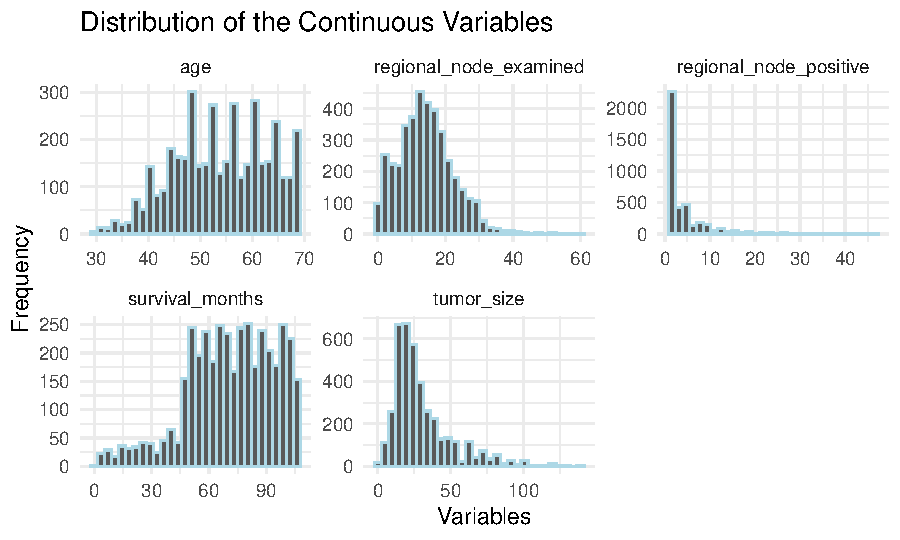
\includegraphics[width=0.9\linewidth]{Appendix_files/figure-latex/distribution_of_the_continuous_variables-1} \caption{Distribution of the Continuous Variables}\label{fig:distribution_of_the_continuous_variables}
\end{figure}

\begin{figure}
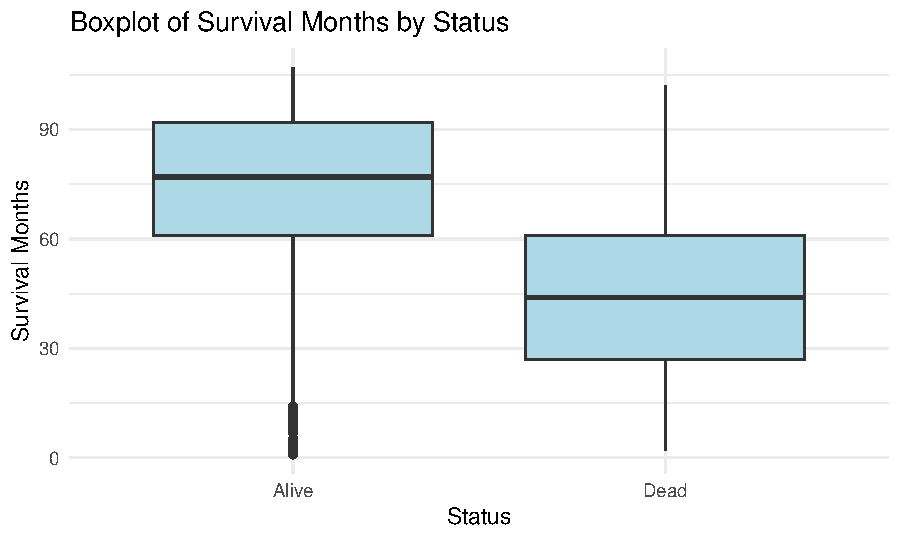
\includegraphics[width=0.9\linewidth]{Appendix_files/figure-latex/survival_months_by_status-1} \caption{Survival Months by Status}\label{fig:survival_months_by_status}
\end{figure}

\begin{figure}
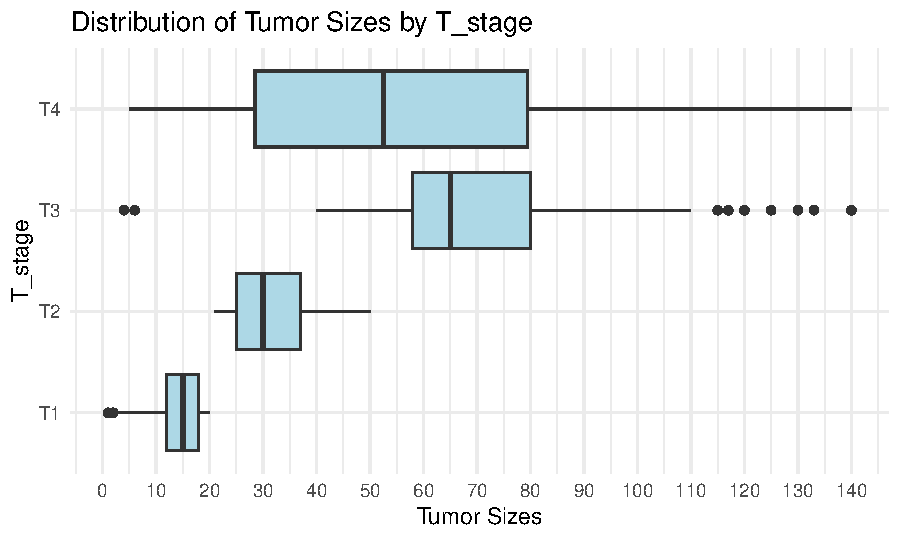
\includegraphics[width=0.9\linewidth]{Appendix_files/figure-latex/tumor_sizes_by_t_stage-1} \caption{Tumor Sizes by T stage}\label{fig:tumor_sizes_by_t_stage}
\end{figure}

\begin{figure}
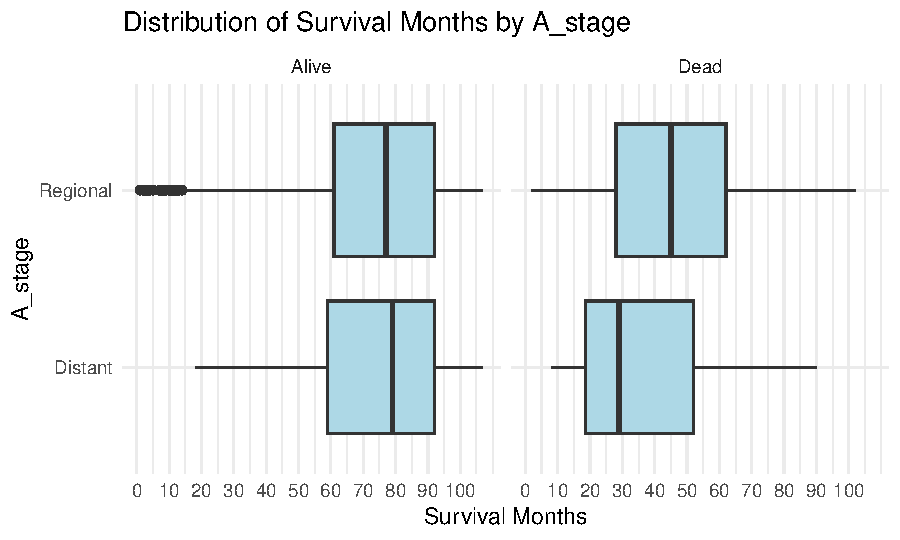
\includegraphics[width=0.9\linewidth]{Appendix_files/figure-latex/survival_months_by_a_stage_based_on_status-1} \caption{Survival Months by A stage Based on Status}\label{fig:survival_months_by_a_stage_based_on_status}
\end{figure}

\begin{figure}
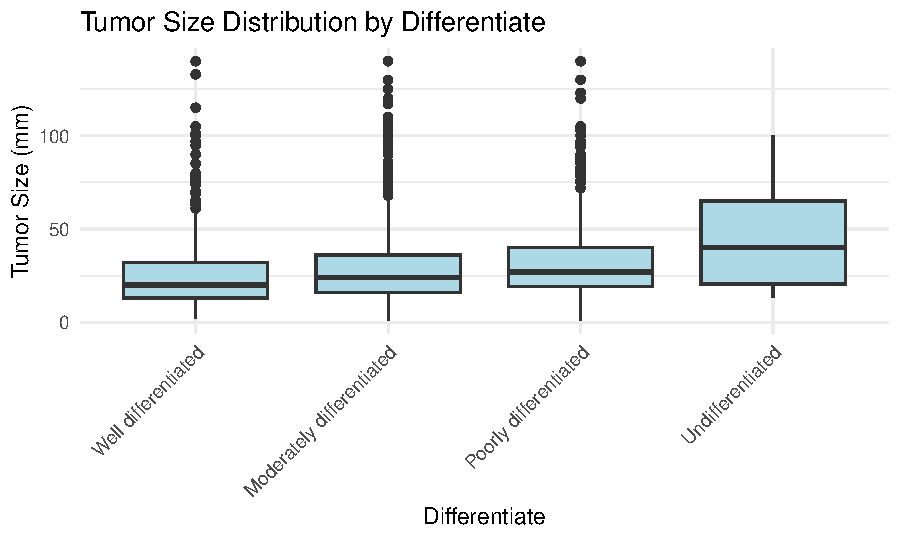
\includegraphics[width=0.9\linewidth]{Appendix_files/figure-latex/tumor_size_by_differentiate-1} \caption{Tumor Size by Differentiate}\label{fig:tumor_size_by_differentiate}
\end{figure}

\begin{figure}
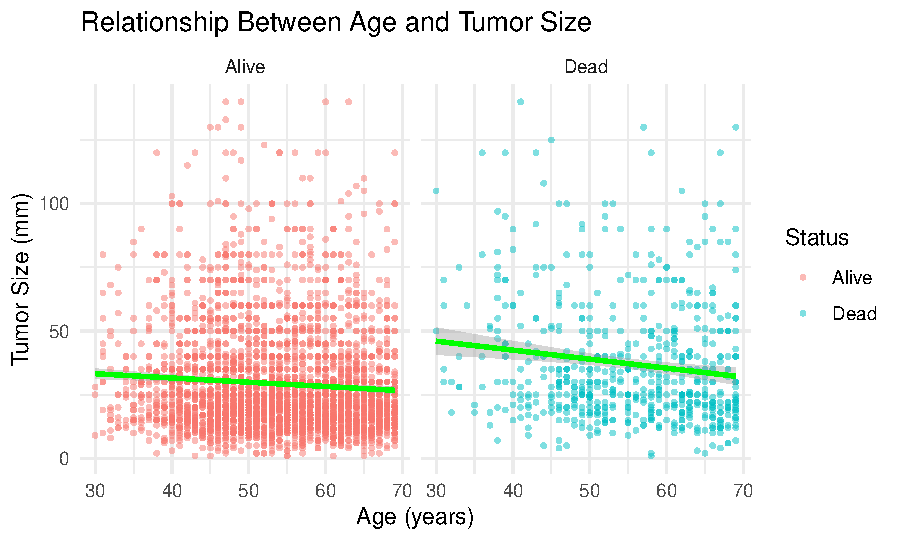
\includegraphics[width=0.9\linewidth]{Appendix_files/figure-latex/relationship_between_age_and_tumor_size_across_status-1} \caption{Relationship Between Age and Tumor Size across Status}\label{fig:relationship_between_age_and_tumor_size_across_status}
\end{figure}

\begin{figure}
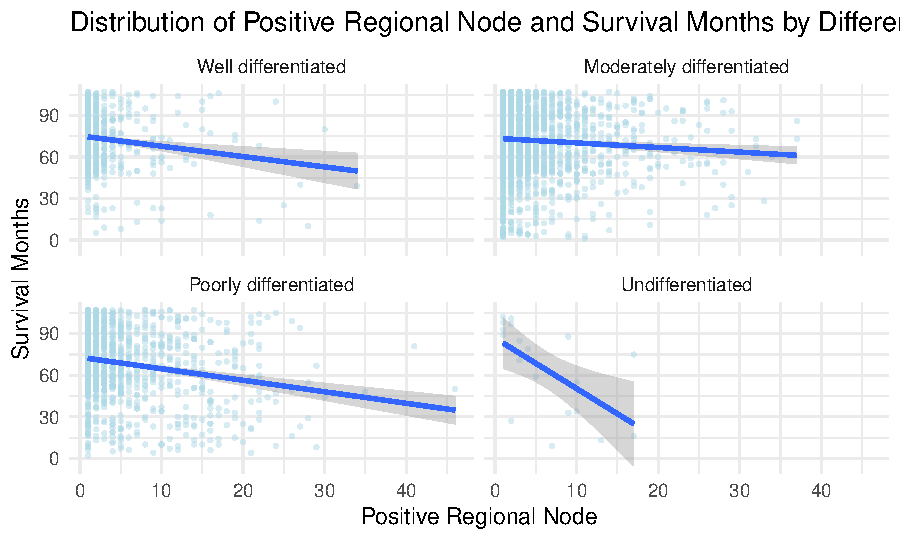
\includegraphics[width=0.9\linewidth]{Appendix_files/figure-latex/positive_regional_node_vs_survival_months_across_differentiate-1} \caption{Positive Regional Node vs Survival Months Across Differentiate}\label{fig:positive_regional_node_vs_survival_months_across_differentiate}
\end{figure}

\newpage

\subsection{Logistic Regression Model}\label{logistic-regression-model}

\subsubsection{Model Selection}\label{model-selection}

\begin{longtable}[]{@{}lrr@{}}
\caption{Model Selection}\tabularnewline
\toprule\noalign{}
type & AIC & BIC \\
\midrule\noalign{}
\endfirsthead
\toprule\noalign{}
type & AIC & BIC \\
\midrule\noalign{}
\endhead
\bottomrule\noalign{}
\endlastfoot
full & 3002.000 & 3159.500 \\
forward & 3002.000 & 3159.500 \\
backward & 2993.771 & 3119.771 \\
stepwise & 2993.771 & 3119.771 \\
\end{longtable}

The Akaike information criterion (AIC) is an estimator of prediction
error and thereby relative quality of statistical models for a given set
of data, and models with lower AIC are generally preferred. Similarly,
the Bayesian information criterion (BIC) is also a criterion for model
selection among a finite set of models. They both resolve the
overfitting problem by introducing a penalty term for the number of
parameters in the model.

By comparing AIC and BIC, we can see the model given by backward
elimination or stepwise regression works slightly better than the full
model or forward selection model. Therefore, we will choose the former
to be our ``best model''.

\subsubsection{Odds Ratios}\label{odds-ratios}

\begin{longtable}[]{@{}
  >{\raggedright\arraybackslash}p{(\columnwidth - 10\tabcolsep) * \real{0.4149}}
  >{\raggedleft\arraybackslash}p{(\columnwidth - 10\tabcolsep) * \real{0.0957}}
  >{\raggedleft\arraybackslash}p{(\columnwidth - 10\tabcolsep) * \real{0.1064}}
  >{\raggedleft\arraybackslash}p{(\columnwidth - 10\tabcolsep) * \real{0.0851}}
  >{\raggedleft\arraybackslash}p{(\columnwidth - 10\tabcolsep) * \real{0.0851}}
  >{\raggedleft\arraybackslash}p{(\columnwidth - 10\tabcolsep) * \real{0.2128}}@{}}
\caption{Final Model Results with Adjusted-Odds Ratio}\tabularnewline
\toprule\noalign{}
\begin{minipage}[b]{\linewidth}\raggedright
\end{minipage} & \begin{minipage}[b]{\linewidth}\raggedleft
estimate
\end{minipage} & \begin{minipage}[b]{\linewidth}\raggedleft
std\_error
\end{minipage} & \begin{minipage}[b]{\linewidth}\raggedleft
z\_value
\end{minipage} & \begin{minipage}[b]{\linewidth}\raggedleft
p\_value
\end{minipage} & \begin{minipage}[b]{\linewidth}\raggedleft
adjusted\_odds\_ratio
\end{minipage} \\
\midrule\noalign{}
\endfirsthead
\toprule\noalign{}
\begin{minipage}[b]{\linewidth}\raggedright
\end{minipage} & \begin{minipage}[b]{\linewidth}\raggedleft
estimate
\end{minipage} & \begin{minipage}[b]{\linewidth}\raggedleft
std\_error
\end{minipage} & \begin{minipage}[b]{\linewidth}\raggedleft
z\_value
\end{minipage} & \begin{minipage}[b]{\linewidth}\raggedleft
p\_value
\end{minipage} & \begin{minipage}[b]{\linewidth}\raggedleft
adjusted\_odds\_ratio
\end{minipage} \\
\midrule\noalign{}
\endhead
\bottomrule\noalign{}
\endlastfoot
(Intercept) & -2.2838 & 0.4385 & -5.2085 & 0.0000 & 0.1019 \\
age & 0.0238 & 0.0056 & 4.2426 & 0.0000 & 1.0241 \\
raceOther & -0.9346 & 0.2485 & -3.7616 & 0.0002 & 0.3928 \\
raceWhite & -0.5148 & 0.1617 & -3.1845 & 0.0014 & 0.5976 \\
marital\_statusMarried & -0.2110 & 0.1416 & -1.4900 & 0.1362 & 0.8097 \\
marital\_statusSeparated & 0.6691 & 0.3881 & 1.7240 & 0.0847 & 1.9526 \\
marital\_statusSingle & -0.0646 & 0.1748 & -0.3696 & 0.7117 & 0.9374 \\
marital\_statusWidowed & 0.0175 & 0.2211 & 0.0791 & 0.9369 & 1.0176 \\
t\_stageT2 & 0.4111 & 0.1130 & 3.6372 & 0.0003 & 1.5085 \\
t\_stageT3 & 0.5516 & 0.1488 & 3.7077 & 0.0002 & 1.7360 \\
t\_stageT4 & 1.0988 & 0.2445 & 4.4934 & 0.0000 & 3.0005 \\
n\_stageN2 & 0.4363 & 0.1284 & 3.3987 & 0.0007 & 1.5470 \\
n\_stageN3 & 0.5872 & 0.2345 & 2.5034 & 0.0123 & 1.7989 \\
differentiateModerately differentiated & 0.5328 & 0.1838 & 2.8990 &
0.0037 & 1.7036 \\
differentiatePoorly differentiated & 0.9190 & 0.1924 & 4.7772 & 0.0000 &
2.5069 \\
differentiateUndifferentiated & 1.8649 & 0.5538 & 3.3672 & 0.0008 &
6.4551 \\
estrogen\_statusPositive & -0.7480 & 0.1775 & -4.2140 & 0.0000 &
0.4733 \\
progesterone\_statusPositive & -0.5842 & 0.1275 & -4.5811 & 0.0000 &
0.5576 \\
regional\_node\_examined & -0.0359 & 0.0072 & -5.0110 & 0.0000 &
0.9647 \\
regional\_node\_positive & 0.0797 & 0.0153 & 5.2076 & 0.0000 & 1.0829 \\
\end{longtable}

\subsubsection{Model Diagnostics}\label{model-diagnostics}

\begin{longtable}[]{@{}lrrr@{}}
\caption{Examination for Multicolinearity}\tabularnewline
\toprule\noalign{}
& GVIF & Df & GVIF\^{}(1/(2*Df)) \\
\midrule\noalign{}
\endfirsthead
\toprule\noalign{}
& GVIF & Df & GVIF\^{}(1/(2*Df)) \\
\midrule\noalign{}
\endhead
\bottomrule\noalign{}
\endlastfoot
age & 1.1072 & 1 & 1.0522 \\
race & 1.0629 & 2 & 1.0154 \\
marital\_status & 1.1291 & 4 & 1.0153 \\
t\_stage & 1.1019 & 3 & 1.0163 \\
n\_stage & 3.8068 & 2 & 1.3968 \\
differentiate & 1.1171 & 3 & 1.0186 \\
estrogen\_status & 1.4754 & 1 & 1.2147 \\
progesterone\_status & 1.4275 & 1 & 1.1948 \\
regional\_node\_examined & 1.4778 & 1 & 1.2157 \\
regional\_node\_positive & 4.2484 & 1 & 2.0612 \\
\end{longtable}

Variance Inflation Factor is a commonly used method for detecting
multicollinearity in regression models. VIF is generally calculated for
the continuous variables, and Generalized Variance Inflation Factor
(GVIF) is used for evaluating the multicollinearity for categorical
variables.

The adjusted GVIF (i.e.~GVIF\^{}(1/(2*Df))) values are corrected for the
degree of freedom and provide a scale similar to VIF. The high adjusted
GVIF values (GVIF \textgreater{} 2) indicate the presence of moderate to
strong multicollinearity.

The table shows that most variables do not show multicollinearity, with
the exception of \texttt{regional\_node\_positive}. Since its adjusted
GVIF is not much different from 2, we will keep this variable for now.

\begin{figure}
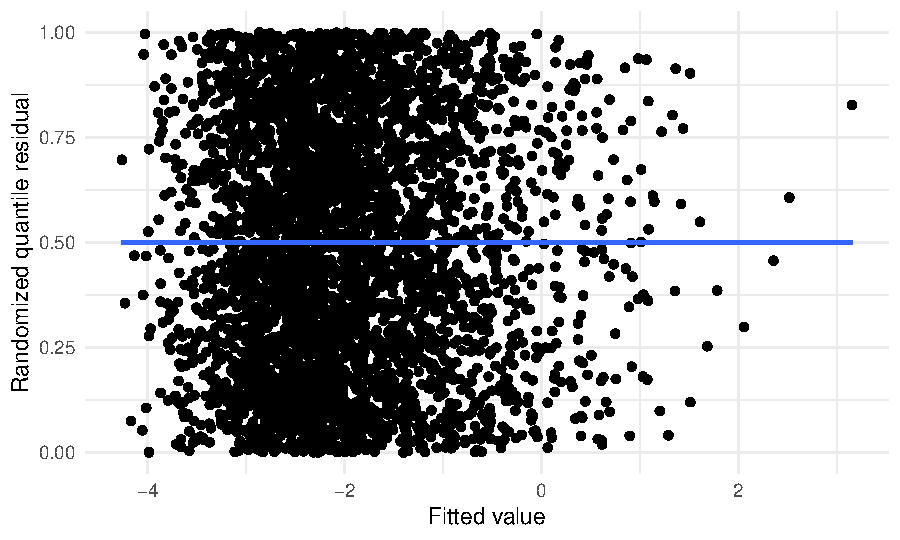
\includegraphics[width=0.9\linewidth]{Appendix_files/figure-latex/unnamed-chunk-6-1} \caption{Random Quantile Residual versus Fitted Values Plot}\label{fig:unnamed-chunk-6}
\end{figure}

By randomizing the quantile residuals, we resolve the problem that the
RVF plot always shows a pattern in logistic regression because of the
binary response variable. Since in the randomized quantile residual
vs.~fitted value plot, the residuals distribute randomly around the 0.5
horizontal line, the residual assumption is met and the model is a good
fit.

\begin{figure}
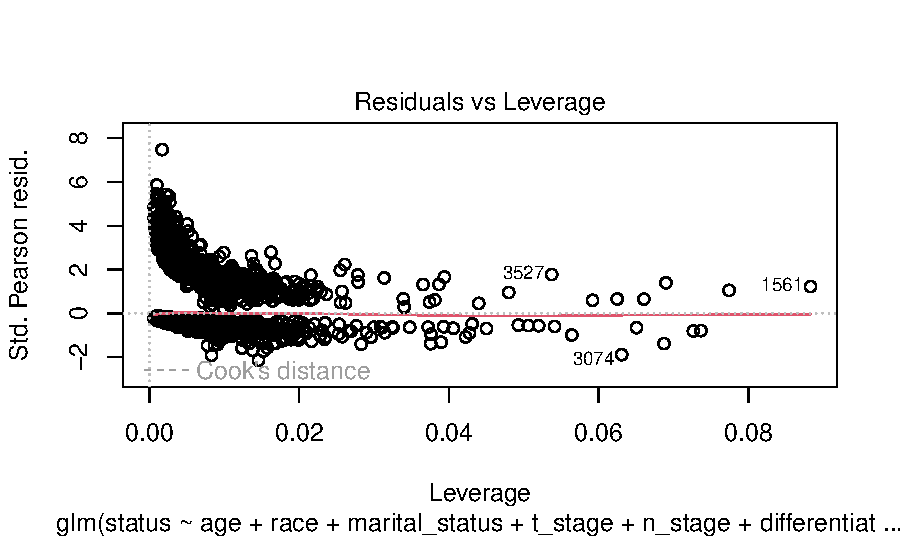
\includegraphics[width=0.9\linewidth]{Appendix_files/figure-latex/unnamed-chunk-7-1} \caption{Residual versus Leverage Plot}\label{fig:unnamed-chunk-7}
\end{figure}

The residual vs.~leverage plot indicates that observations 3527, 1561,
and 3074 may be potential outliers, but they are not necessarily
influential.

\newpage

\subsubsection{Cross Validation}\label{cross-validation}

\begin{longtable}[]{@{}rr@{}}
\caption{Results of 10-Fold Cross Validation}\tabularnewline
\toprule\noalign{}
log\_loss & AUC \\
\midrule\noalign{}
\endfirsthead
\toprule\noalign{}
log\_loss & AUC \\
\midrule\noalign{}
\endhead
\bottomrule\noalign{}
\endlastfoot
0.3681 & 0.6999 \\
0.3639 & 0.7463 \\
0.4069 & 0.7498 \\
0.3773 & 0.7552 \\
0.3575 & 0.7792 \\
0.3780 & 0.7317 \\
0.3679 & 0.6604 \\
0.3636 & 0.7951 \\
0.3681 & 0.7644 \\
0.3718 & 0.7405 \\
\end{longtable}

After applying 10-fold cross-validation, we evaluate the goodness of fit
by log loss and AUC. The mean of log loss is 0.3723182, and the mean of
AUC is 0.7422428.

\subsubsection{Evaluation Across Races}\label{evaluation-across-races}

\begin{longtable}[]{@{}lrr@{}}
\caption{Race Comparison Before Adding Interaction Terms}\tabularnewline
\toprule\noalign{}
race & avg\_log\_loss & avg\_AUC \\
\midrule\noalign{}
\endfirsthead
\toprule\noalign{}
race & avg\_log\_loss & avg\_AUC \\
\midrule\noalign{}
\endhead
\bottomrule\noalign{}
\endlastfoot
Black or other & 0.4231 & 0.6997 \\
White & 0.3651 & 0.7502 \\
\end{longtable}

Low log loss and high AUC indicate better test performance.

To reduce the gap of prediction performance between the majority and
minority, we focused on whether there were interactions between the
variables. We extracted each variable from the best model and examined
how it differed in survival months of survival by race. Most variables
did not show significant differences by race, suggesting that there may
not be an interaction between these variables and race. However, the
variable marital status showed a different pattern.

\begin{figure}
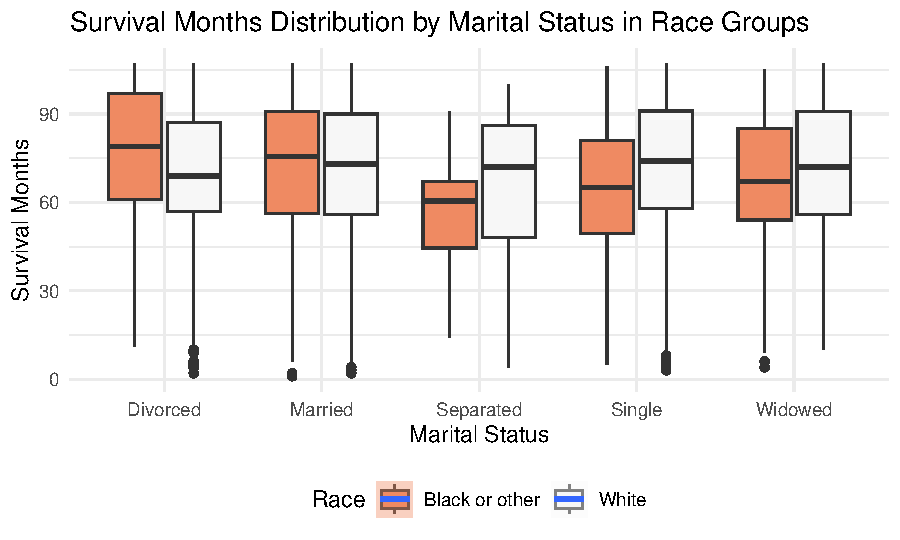
\includegraphics[width=0.9\linewidth]{Appendix_files/figure-latex/race_inter_marital-1} \caption{Survival Months Distribution by Marital Status in Race Groups}\label{fig:race_inter_marital}
\end{figure}

From the figure we can see that the distribution of survival months is
different between races with different marital status. This indicates
the potential interaction between race and marital status, and the
interaction term can be added in the model to improve the fairness of
the model.

\begin{longtable}[]{@{}lrr@{}}
\caption{Race Comparison After Adding Interaction Terms}\tabularnewline
\toprule\noalign{}
race & avg\_log\_loss & avg\_AUC \\
\midrule\noalign{}
\endfirsthead
\toprule\noalign{}
race & avg\_log\_loss & avg\_AUC \\
\midrule\noalign{}
\endhead
\bottomrule\noalign{}
\endlastfoot
Black or other & 0.4169 & 0.7251 \\
White & 0.3647 & 0.7501 \\
\end{longtable}

By adding interaction term \texttt{marital\_status\ *\ race}, we can
observe a decrease in log loss and an increase in AUC, which means an
improve in the fairness between group ``White'' and the minority
``Black'' + ``Other''.

\newpage

\subsection{Survival Analysis}\label{survival-analysis}

\subsubsection{Kaplan Meier Curve}\label{kaplan-meier-curve}

The Kaplan Meier curve graphically represent the survival rate. Time is
plotted on the x-axis and the survival rate is plotted on the y-axis.

\begin{figure}
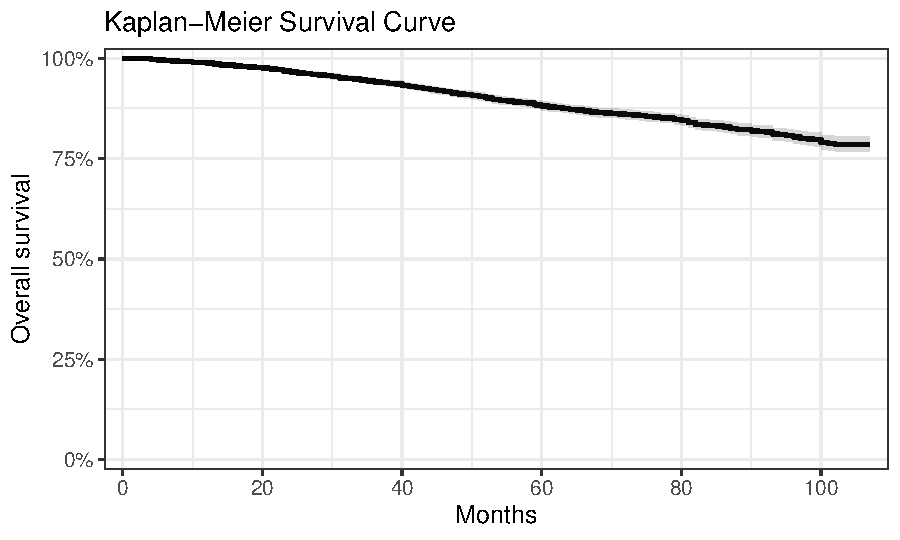
\includegraphics[width=0.9\linewidth]{Appendix_files/figure-latex/km_curve-1} \caption{Kaplan-Meier Survival Curve}\label{fig:km_curve}
\end{figure}

\subsubsection{Log Rank Test}\label{log-rank-test}

The log rank test lets us test whether there is a difference in survival
times between groups of patients. For example, we want to find out
whether there is a significant difference in survival between patients
whose cells have different degrees of differentiation.

\begin{figure}
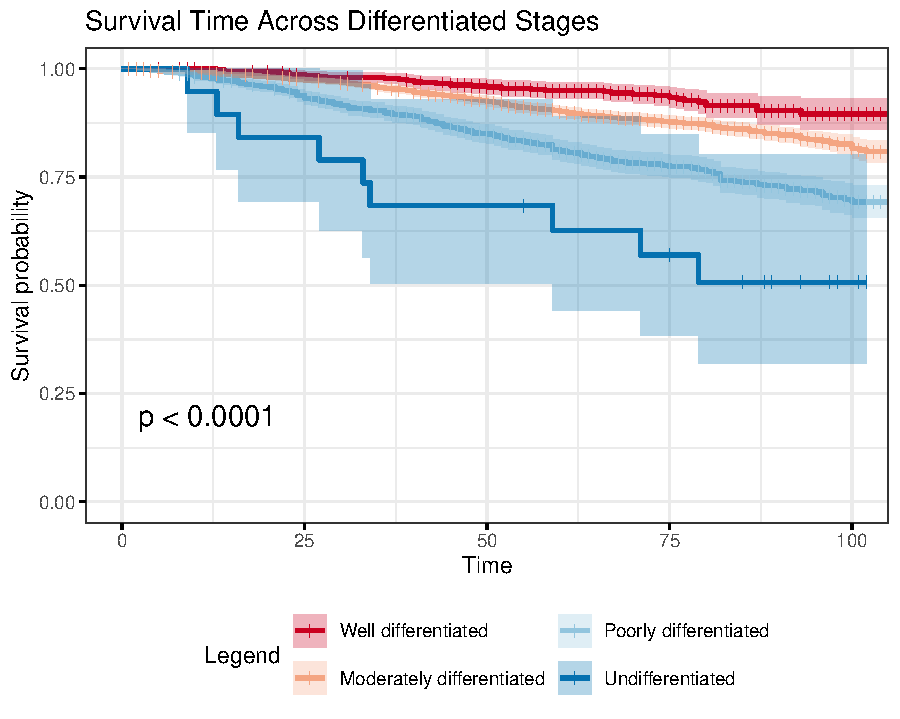
\includegraphics[width=0.9\linewidth]{Appendix_files/figure-latex/log_rank-1} \caption{Survival Time Across Differentiated Stages}\label{fig:log_rank}
\end{figure}

\newpage

\subsubsection{Cox Model}\label{cox-model}

The limitation of KM curves and log-rank tests is that we can only test
one variable at a time. To further discuss the risk factors to survival
time, we will compute the cox proportional hazard model to adjusts for
multiple risk factors simultaneously.

The cox proportional hazard model has a assumption: the survival curves
for two different strata of a risk factor must have hazard functions
that are proportional over time. This assumption is satisfied when the
change in hazard from one category to the next does not depend on time.
That is, a person in one stratum has the same instantaneous relative
risk compared to a person in a different stratum, irrespective of how
much time has passed.

We will test this assumption based on the scaled Schoenfeld residuals.
Here is an interpretation of the results: When p-val \textless{} 0.05,
there is evidence against the proportional hazards assumption, meaning
that the HR is not constant over time. Similarly, the larger the
chi-square value, the greater the violation of the assumption.

\begin{longtable}[]{@{}lrrr@{}}
\caption{Results of Cox Proportional Hazard Model}\tabularnewline
\toprule\noalign{}
& chisq & df & p \\
\midrule\noalign{}
\endfirsthead
\toprule\noalign{}
& chisq & df & p \\
\midrule\noalign{}
\endhead
\bottomrule\noalign{}
\endlastfoot
age & 0.1328 & 1 & 0.7156 \\
race & 0.9335 & 2 & 0.6270 \\
marital\_status & 2.6670 & 4 & 0.6150 \\
t\_stage & 0.2144 & 3 & 0.9752 \\
n\_stage & 1.7178 & 2 & 0.4236 \\
x6th\_stage & 3.8545 & 3 & 0.2776 \\
differentiate & 1.8899 & 3 & 0.5956 \\
a\_stage & 5.2218 & 1 & 0.0223 \\
tumor\_size & 0.9310 & 1 & 0.3346 \\
estrogen\_status & 28.9294 & 1 & 0.0000 \\
progesterone\_status & 32.1281 & 1 & 0.0000 \\
regional\_node\_examined & 0.0187 & 1 & 0.8912 \\
regional\_node\_positive & 0.0324 & 1 & 0.8571 \\
GLOBAL & 57.2155 & 24 & 0.0002 \\
\end{longtable}

We can see from the table that variable \texttt{a\_stage},
\texttt{estrogen\_status}, \texttt{progesterone\_status} are not
constant over time, which means it's not proper to contain these
covariates in cox regression. To reduce bias of the model, we can remove
these variables and take a closer look at the result.

\begin{figure}
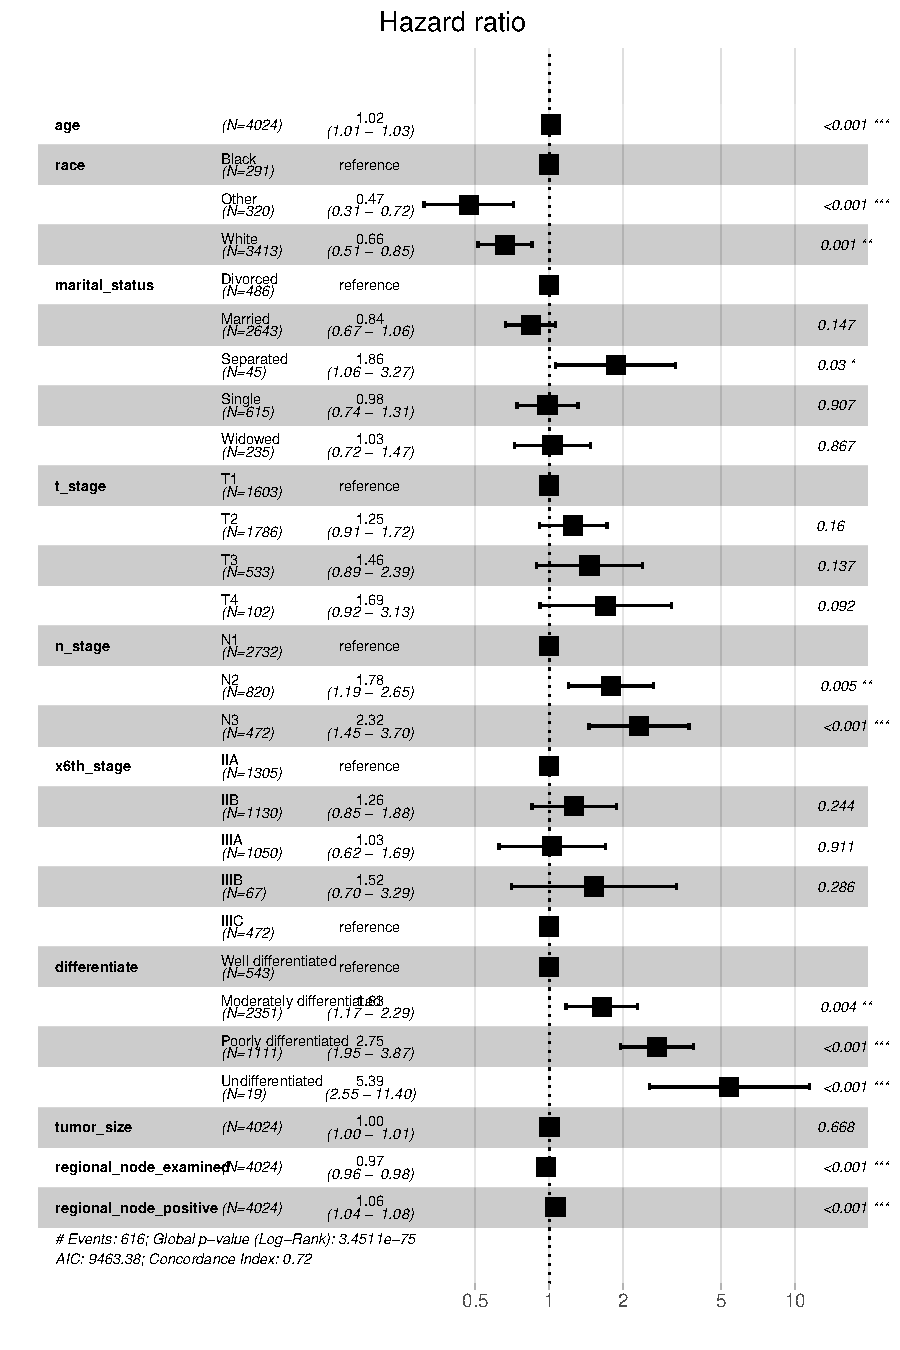
\includegraphics[width=1\linewidth]{Appendix_files/figure-latex/forest_plot-1} \caption{Forest Plot of Hazard Ratios}\label{fig:forest_plot}
\end{figure}

The hazard ratio is similar to relative risk, but differs in that the HR
is the instantaneous risk rather than the cumulative risk over the
entire study.

The x-axis of this forest plot represents hazard ratios. Hazard ratio =
1 means no significant difference compared to the reference, and a HR
higher than 1 means it increases the hazard ratio of the event, death,
and a HR lower than 1 decreases it. The smaller the p-value is the
stronger the weight of evidence that the two groups are different.

We can conclude from the plot that for the variable race, blacks have
the highest hazard of death, followed by whites, while the lowest
mortality rate is for other ethnic groups. In the variable marital
status, the hazard of death is significantly higher for separated
people, but this may be due to information bias caused by fewer
observations. The confidence intervals for the other categories of
marital status all contain the null hypothesis, meaning that there is no
significant difference.

The hazard of death is highest for patients with N stage N3, followed by
N2, and finally N1. Differently, although T stage also shows a similar
trend, the confidence intervals of each stage level contain the null
hypothesis, meaning that there is no significant difference between
levels. For the 6th stage, IIIB has the highest hazard of death,
followed by IIB, and then IIA, but there is no significant difference.
For stage IIIC, since it contains the same information as N3 of N stage,
no comparison is made in this variable.

In the variable differentiated, the hazard of death is significantly
highest for undifferentiated, and then decreases in the order of poorly
differentiated, moderately differentiated, and well differentiated.

For the variables tumor size, regional node examined, and regional node
postive, we did not observe significant differences in the hazard of
death.

\end{document}
